\documentclass[aspectratio=169]{beamer} % Set 16:9 aspect ratio
\usepackage{graphicx}
\usepackage{hyperref}
\usepackage{xcolor} % Add xcolor package

% Define custom dark blue color
\definecolor{darkblue}{RGB}{0, 0, 139} 

\usecolortheme{seahorse} % Enhances contrast for dark backgrounds
\setbeamercolor{background canvas}{bg=darkblue} % Sets background to dark blue
\setbeamercolor{normal text}{fg=white} % Sets all text to white
\setbeamercolor{structure}{fg=white} % Ensures headings and lists are white

% Remove navigation symbols
\setbeamertemplate{navigation symbols}{} 

\title{Exploring Solar Panel Efficiency}
\author{Eliott Hall}
\date{} % Remove the date

\begin{document}

\frame{\titlepage}

% Introduction Slide
\begin{frame}{Introduction}
    \textbf{Limits are to be pushed.}
    \begin{itemize}
        \item What is the maximum possible efficiency of a solar panel?
        \item Costs and financial feasibility.
    \end{itemize}
\end{frame}

% Part 1: Theoretical Limits
\begin{frame}{Theoretical Limits of Solar Efficiency}
    \textbf{Physics sets fundamental constraints on efficiency:}
    \begin{itemize}
        \item \textbf{Shockley-Queisser Limit}: Max efficiency of a single-junction silicon cell is about 33.7\%.
        \item \textbf{Multijunction Solar Cells}: Up to 86% efficiency.
        \item \textbf{Quantum Dot Technology}: Potential for even higher efficiencies.
    \end{itemize}
    \centering
    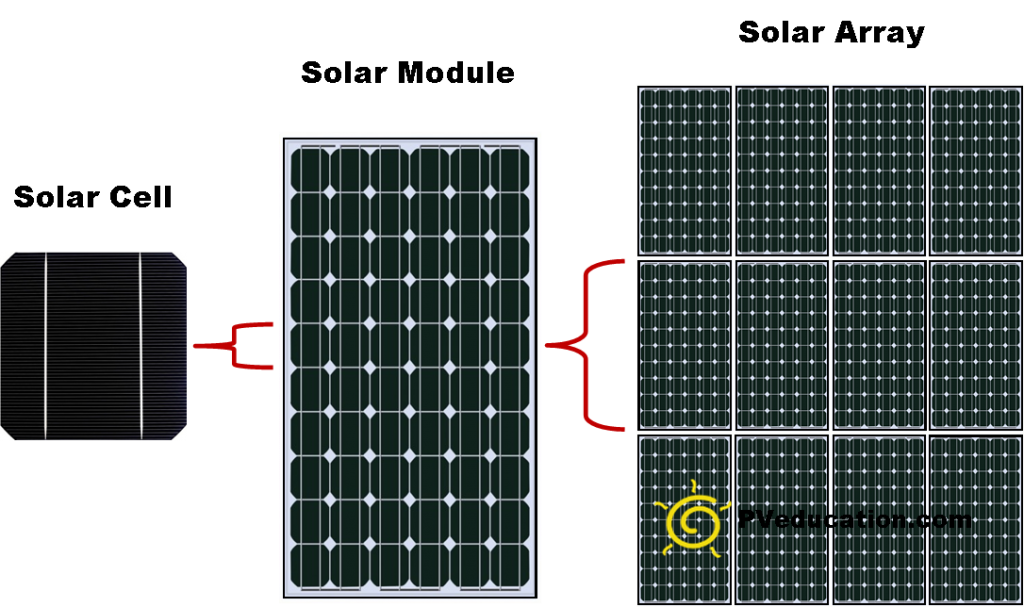
\includegraphics[width=0.7\linewidth]{solar_cells.png} % Add relevant image
\end{frame}

% Part 2: Cost and Feasibility
\begin{frame}{Cost and Financial Feasibility}
    \textbf{High efficiency comes at a cost:}
    \begin{itemize}
        \item \textbf{Multijunction Solar Cells}: Over \$100,000 per square meter.
        \item \textbf{Standard Silicon Panels}: \$150--\$400 per panel, 15--22\% efficiency.
        \item \textbf{Emerging Perovskite Cells}: 30--35\% efficiency at lower costs.
    \end{itemize}
    \centering
    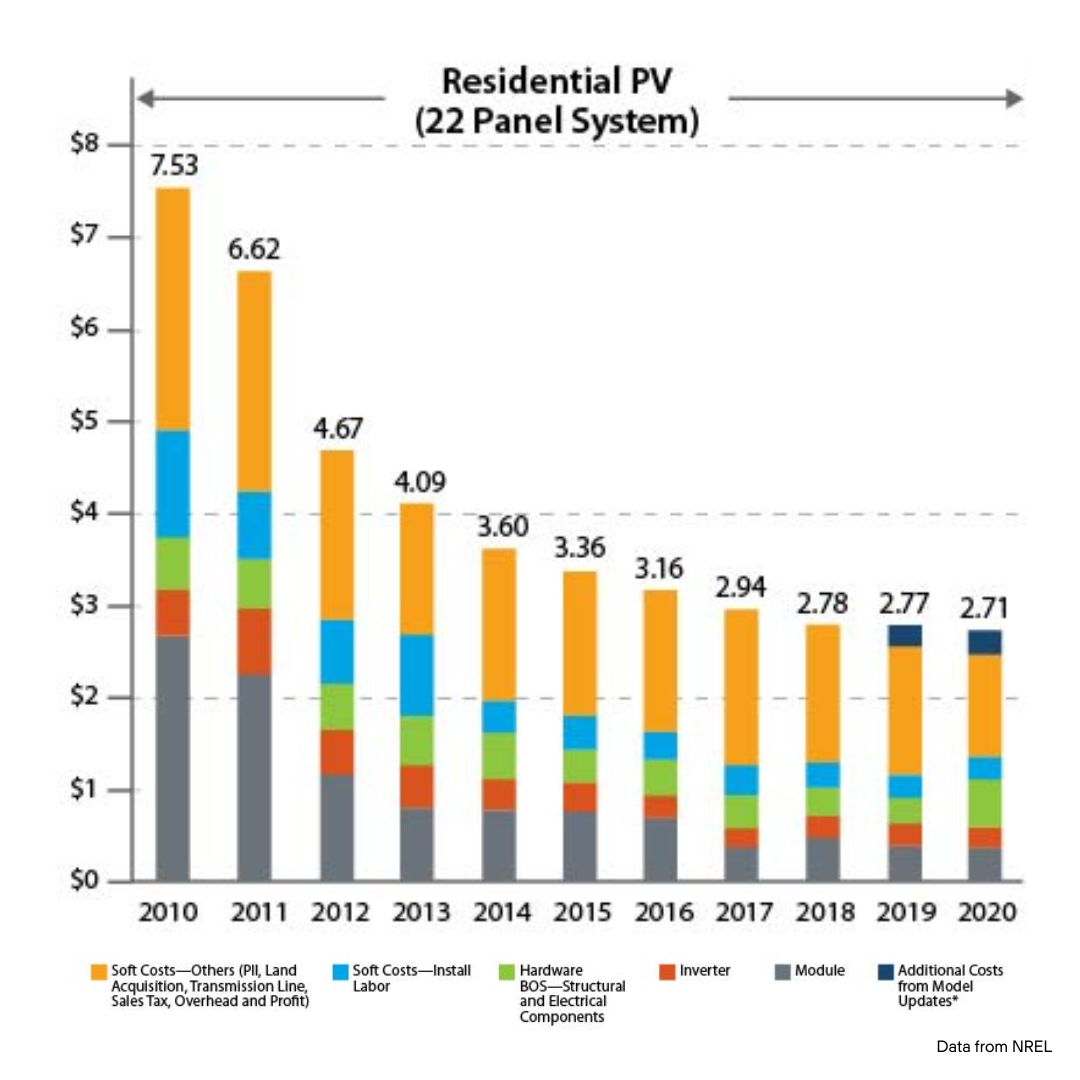
\includegraphics[width=0.6\linewidth]{solar_costs.png} % Add relevant image
\end{frame}

% Conclusion Slide
\begin{frame}{Conclusion}
    \textbf{Balancing Efficiency, Cost, and Practicality}
    \begin{itemize}
        \item Theoretical efficiency is not easily achievable.
        \item Must optimize cost.
        \item The future is in balancing efficiency and cost.
    \end{itemize}
\end{frame}

\end{document}
